% vim:ft=tex: %
\documentclass[dvipdfmx,uplatex,11pt]{beamer}
\usepackage{bxdpx-beamer}
\usepackage{amsthm} %theolem
\usepackage{amsmath} %\eqref \text
\usepackage{amssymb}
\usepackage{bm}
\usepackage{svg}
\usepackage{mathtools}
\mathtoolsset{showonlyrefs}
\theoremstyle{definition}
\newtheorem{define}{定義}
\newtheorem{algorithm}{アルゴリズム}
% \newtheorem{problem}{問題}
\newtheorem{lemmma}{補題}
\newtheorem{theolem}{定理}
\newtheorem{proposition}{命題}
% \newtheorem{example}{例}
% \newcommand{\defpro}{\overset{\mathrm{def}}{\Leftrightarrow}}
%\DeclareFontShape{JY1}{mc}{m}{it}{<5> <6> <7> <8> <9> <10> sgen*min
    %<10.95><12><14.4><17.28><20.74><24.88> min10 <-> min10}{}
%\DeclareFontShape{JT1}{mc}{m}{it}{<5> <6> <7> <8> <9> <10> sgen*tmin
    %<10.95><12><14.4><17.28><20.74><24.88> tmin10 <-> tmin10}{}
\DeclareFontShape{JY2}{mc}{m}{it}{<5> <6> <7> <8> <9> <10> sgen*min
    <10.95><12><14.4><17.28><20.74><24.88> min10 <-> min10}{}
\DeclareFontShape{JT2}{mc}{m}{it}{<5> <6> <7> <8> <9> <10> sgen*tmin
    <10.95><12><14.4><17.28><20.74><24.88> tmin10 <-> tmin10}{}
\renewcommand\proofname{\bf 証明}
\usepackage[deluxe,expert]{otf}
\usefonttheme{structurebold} % タイトル部を太字
\setbeamerfont{alerted text}{series=\bfseries} % Alertを太字
\setbeamerfont{section in toc}{series=\mdseries} % 目次は太字にしない
\setbeamerfont{frametitle}{size=\Large} % フレームタイトル文字サイズ
\setbeamerfont{title}{size=\LARGE} % タイトル文字サイズ
\setbeamerfont{date}{size=\small}  % 日付文字サイズ

% Babel (日本語の場合のみ・英語の場合は不要)
\uselanguage{japanese}
\languagepath{japanese}
\deftranslation[to=japanese]{Theorem}{定理}
\deftranslation[to=japanese]{Lemma}{補題}
\deftranslation[to=japanese]{Example}{例}
\deftranslation[to=japanese]{Examples}{例}
\deftranslation[to=japanese]{Definition}{定義}
\deftranslation[to=japanese]{Definitions}{定義}
\deftranslation[to=japanese]{Problem}{問題}
\deftranslation[to=japanese]{Solution}{解}
\deftranslation[to=japanese]{Fact}{事実}
\deftranslation[to=japanese]{Proof}{証明}
\renewcommand{\kanjifamilydefault}{mg}
\setbeamertemplate{footline}[frame number] 
\usepackage{algorithm}
\usepackage[noend]{algorithmic}
\usepackage{graphicx}
\title{シミュレーションの高速化と精度向上技術の調査}
\subtitle{シミュレーションの並列処理とデータ同化}
\author{和田 篤}
\date{\today}
\usetheme{Berkeley}

\begin{document}
\begin{frame}
  \maketitle
\end{frame}

\begin{frame}{動機と狙い}

  \begin{block}{テーマ選択理由}
   \begin{itemize}
      \item シミュレーションの精度を上げたい,計算時間を短くしたいという声をよく聞く
      \item 得意分野の機械学習,アルゴリズムでシミュレーション技術に貢献したい
    \end{itemize}
  \end{block}

  \begin{block}{狙い}
   \begin{itemize}
      \item 並列化とデータ同化技術のアイデアと基本を紹介し,技術開発方針検討の一助に
    \end{itemize}
  \end{block}

\end{frame}

\begin{frame}{目次}
  \tableofcontents
\end{frame}

\section{離散イベントシミュレーション}
\subsection{問題}
\begin{frame}{シミュレーションの分類}
  \begin{block}{状態変化の数による分類}

    \begin{itemize}
      \item 連続ミュレーション:  状態変化が無限回
      \item 離散イベントシミュレーション:  状態変化が有限回
    \end{itemize}
  \end{block}

  \begin{columns}
  
    \begin{column}{0.5\textwidth}
      
      \begin{figure}[htb]
        \centering
        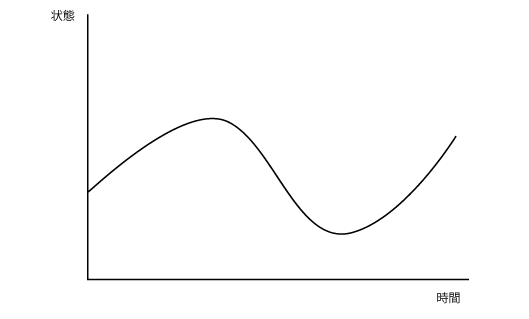
\includegraphics[scale=0.3]{continuous_sim.png}
        \caption{ \small 連続シミュレーション}
      \end{figure}
    \end{column}

    \begin{column}{0.5\textwidth}
      
      \begin{figure}[htb]
        \centering
      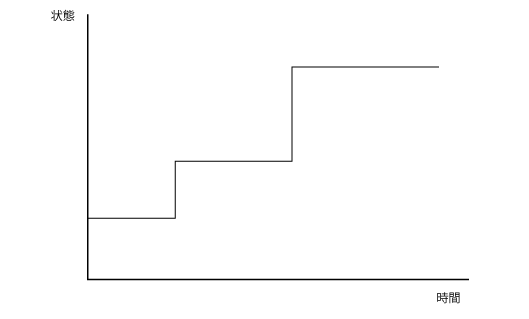
\includegraphics[scale=0.3]{discrete_sim.png}
        \caption{\small 離散シミュレーション}
      \end{figure}
    \end{column}
  
  \end{columns}
\end{frame}

\begin{frame}{離散イベントシミュレーション(DES)}
  \begin{block}{DESの主要構成要素}
  \begin{description}
      \small
    \item[時刻] シミュレーション上の時刻
    \item[状態] シミュレーションで計算したい値
    \item[イベント] 状態を変化させる \& 新たなイベントを生成
  \end{description}
\end{block}

\begin{columns}
\begin{column}{0.4\textwidth}
 \begin{figure}
   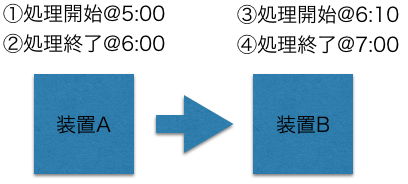
\includegraphics[scale=0.3]{sim.png}
   \caption{DESの例}
  \end{figure}
\end{column}

  \begin{column}{0.6\textwidth}

  \tiny
    \begin{table}
      \caption{DESの例(詳細)}
      \begin{tabular}{ccc}
        時刻 & イベント & 状態\\
        4:00 & DES開始 & \{\}    \\
        5:00 & ① & \{装置A: 処理中\} \\
        6:00 & ② & \{装置A工数:1\} \\
        6:10 & ③ & \{装置A工数:1,装置B: 処理中\} \\
        7:00 & ④& \{装置A工数:1,装置B工数: 1\} \\
        8:00 & DES終了 & \{装置A工数:1,装置B工数: 1\} 
      \end{tabular}
    \end{table}
  \end{column}
\end{columns}

\end{frame}

\subsection{アルゴリズム}
\begin{frame}{DESに対するアルゴリズム: time-bucket法}
  \begin{block}{time-bucket法(単位時間ごとに計算)}
    単位時間を定義し,単位時間ごとに処理すべきイベントがあるか確認する.
    \begin{algorithmic}[1]
      \WHILE{終了条件を満たさない}
      \STATE 時刻を単位時間すすめる
      \IF{現在時刻に処理すべきイベントがある}
        \STATE イベントを処理する.
      \ENDIF
      \ENDWHILE
    \end{algorithmic}
  \end{block}

  \begin{figure}[htb]
    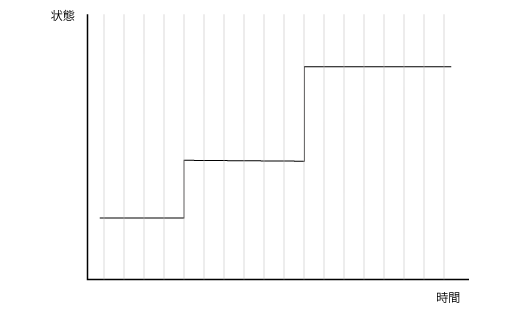
\includegraphics[scale=0.25]{continuous_sim_time_bucket.png}
    \caption{time-bucket法のイメージ}
  \end{figure}

\end{frame}
      %%\\ 発生可能時刻が付随する.
    %%\item[イベント] ある時刻に状態を変化させる \& 新規イベントを生成. 
    %%\item[イベントキュー] イベントを保持するコンテナ.イベントの発生可能時刻によって保持する要素をソートする.

%%\begin{column}{0.5\textwidth}
  %%\begin{table}
    %%\caption{DESの例(詳細)}
    %%\begin{tabular}{ccc}
      %%%%時刻 & イベント & イベントキュー\\
      %%-1 & DES開始 & ①  &  \\
      %%0 & ① & ②
      %%5 & ② & ③
      %%5 & ③ & ④
      %%1 & ④kkkk & B
      %%1 & A & B
    %%\end{tabular}
  %%\end{table}
%%\end{column}
%%\end{columns}

\begin{frame}{DESに対するアルゴリズム: event-driven法}
  \begin{block}{event-driven法(状態変化時のみ計算)}
    イベントキューを利用して,イベントが発生する時刻のみ計算する.
    \begin{algorithmic}[1]
      \WHILE{終了条件を満たさない}
      \STATE イベントキューの先頭にあるイベントを処理
      \STATE 時刻を取り出したイベントの発生時刻にする
      \STATE イベントを処理する
      \ENDWHILE
    \end{algorithmic}
  \end{block}

  \begin{figure}[htb]
    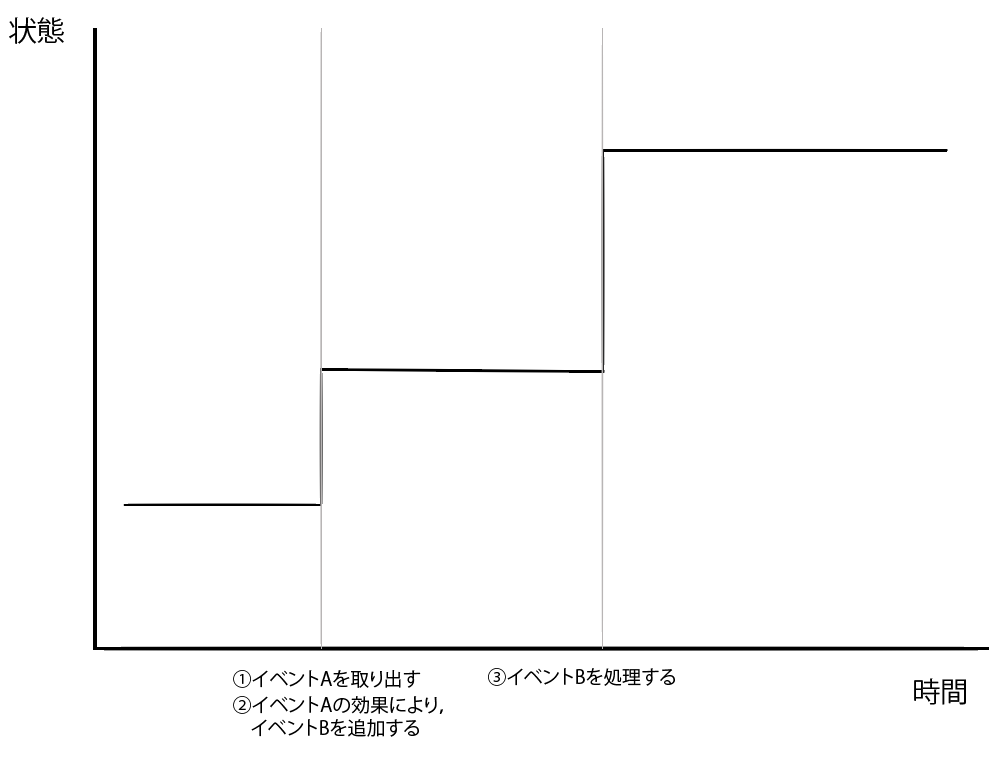
\includegraphics[scale=0.1]{event_driven_method.png}
    \caption{event-driven法のイメージ}
  \end{figure}

\end{frame}
\section{並列処理}

\subsection{悲観的な方法}

\begin{frame}{Parallel DESの基本アイデア}
  \begin{block}{アイデア}
    \begin{itemize}
      \item 生産シミュレーションにおいて,別々の装置は並列に処理できるのではないか?
      \item 待ち行列シミュレーションにおいて,別々のサービスは並列に処理できるのではないか?
    \end{itemize}
  \end{block}
  \begin{columns}
    \begin{column}{0.5\textwidth}
      \begin{figure}[htb]
        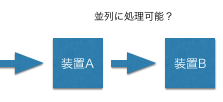
\includegraphics[scale=0.5]{machine_para.png}
      \caption{生産シミュレーションの並列化}
      \end{figure}
    \end{column}
    \begin{column}{0.5\textwidth}
      \begin{figure}
        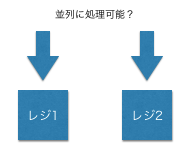
\includegraphics[scale=0.5]{queue_para.png}
        \caption{待ち行列シミュレーションの並列化}
      \end{figure}
    \end{column}
  \end{columns}
\end{frame}

\begin{frame}{基本概念}
  \begin{block}{基本概念}
    \small
    \begin{description}
      \item[LogicalProcess] イベントを処理する仮想エンティティ.それぞれのLogicalProcessが状態を持つ.
      \item[イベント] 1つのLogicalProcessで発生し,そのLogicalProcessの状態のみ変化させる.
      \item[メッセージ] イベントが発生した際に,他のLogicalProcessに送信するイベントのこと.
    \end{description}
  \end{block}
  \begin{figure}
    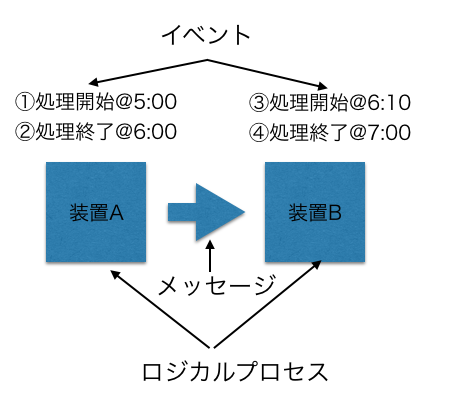
\includegraphics[scale=0.2]{basic_idea.png}
    \caption{生産シミュレーションの例}
  \end{figure}
\end{frame}


\begin{frame}{並列処理可能}
  \begin{block}{並列処理可能}
  Q: どんな時に並列に処理しても結果が変わらないか? \\
  A: 各ロジカルプロセスのイベントを処理する順序が並列処理しない場合と変わらなければOK.
  \end{block}
\end{frame}

\begin{frame}{ネットワークモデル}
  \begin{block}{ネットワークの定義}
    \begin{description}
      \item[node] ロジカルプロセス
      \item[edge] nodeAからnodeBにメッセージを一度でも送る場合nodeAからnodeBに枝をはる.
      \item[edge's weight] これまでにその枝をを通しておくられたメッセージの最大時刻.
    \end{description}

  \end{block}
\end{frame}

\begin{frame}{並列処理可能である十分条件}
  \begin{block}{アイデア}
    \begin{itemize}
      \item 他のロジカルプロセスから送られてくる可能性のあるイベントを処理すべき時刻の最小時刻より,小さければ処理してOK.
      \item 各ロジカルプロセスからロジカルプロセスへのメッセージ
            時間が単調増加だと仮定する
          \item nodeAへ接続している枝の重みが最小の時刻もしくは最小時刻より小さい時刻のイベントは処理してOK
    \end{itemize}

  \end{block}
\end{frame}

\begin{frame}{null-message}
  \begin{block}{課題}
    あまりメッセージを送らない場合edge's weightが更新されず,
    並列処理の効率が下がる.
  \end{block}
  \begin{block}{解決方法}
    null-message(状態を変化させないメッセージ)を送信する.
  \end{block}
\end{frame}

\subsection{楽観的な方法}
\begin{frame}{time-warp法の動機}
  \begin{block}{悲観的な方法の課題}
    \begin{itemize}
  \item 悲観的な方法では,確実に安全な場合しか並列処理できない
  \item null-messageを多用した場合, 並列処理率は高まるが,オーバーヘッドが増える
\end{itemize}
  \end{block}

  \begin{block}{time-warp法のアイデア}
  time-warp法では安全でなくてもまず並列に処理し,
  イベントを処理する順序を間違えていたことがわかった際にrollbackする.a
  \end{block}

\end{frame}

\begin{frame}{rollback}
  \begin{block}{rollbackするタイミング}
    届いたメッセージがすでに処理したイベントより前の時刻だったとき.
  \end{block}
  \begin{block}{イベントの作用}
  \begin{itemize}
    \item LPの状態を変化させる
    \item 他のLPにメッセージを送信する
  \end{itemize}
  \end{block}
  \begin{block}{ロールバックの種類}
    \begin{description}
      \item[restolation] LogicalProcesの状態をロールバック
      \item[antimessage] 他のLogicalProcesに送ったメッセージをキャンセル
  \end{description}
  \end{block}
\end{frame}

\begin{frame}{restolation}
  \begin{block}{状態を保存}
    restolationではLogicalProcessを過去の状態に戻れるようにしておく必要がある.
    そこで,状態を変化させる際には変化前の状態も保存しておく.
  \end{block}
\end{frame}

\begin{frame}{antimessage}
  \begin{block}{antimessageの作用分類}
    \begin{description}
      \item[メッセージ未処理] メッセージを消去する
      \item[メッセージ処理済み]メッセージを処理した時間までリストアする
    \end{description}
  \end{block}
\end{frame}

\section{データ同化}
 \subsection{三次元データ同化}
 \subsection{四次元データ同化}
\begin{frame}{動機}
  a
\end{frame}

\begin{thebibliography}{n}
  \bibitem{PEDS} Fujimoto, Richard M. "Parallel discrete event simulation." Communications of the ACM 33.10 (1990): 30-53.
  \bibitem{PEDSbook} Fujimoto, Richard M. Parallel and distributed simulation systems. Vol. 300. New York: Wiley, 2000.
  \bibitem{time-warp} Jefferson, David, and Henry A. Sowizral. "Fast concurrent simulation using the time warp mechanism." (1982).
  \bibitem{time-link} Chandy, K. Mani, and Jayadev Misra. "Distributed simulation: A case study in design and verification of distributed programs." IEEE Transactions on software engineering 5 (1979): 440-452.
\end{thebibliography}
\end{document}

